\section{Anhang}

\subsection{Einleitung}
\subsubsection{Blockdiagramm}
\begin{figure}[htbp]
	\centering
	\includegraphics[width=0.8\textwidth]{8_Anhang/Blockdiagramm.png}
	\caption{Blockdiagramm vom CanSat}
	\label{blockdiagramm}
\end{figure}

\newpage

\subsection{GANTT-Diagramme}
\subsubsection {Hardware-GANTT}
\begin{figure}[H]
	\centering
	\includegraphics[trim = 2mm 2mm 2mm 2mm, clip,width=0.8\textwidth]{8_Anhang/hardware-gantt-1.png}
	\caption{Das GANTT-Diagramm der Hardware}
	\label{gantt_hardware}
\end{figure}

\subsubsection {Bodenstation-GANTT}
\begin{figure}[H]
	\centering
	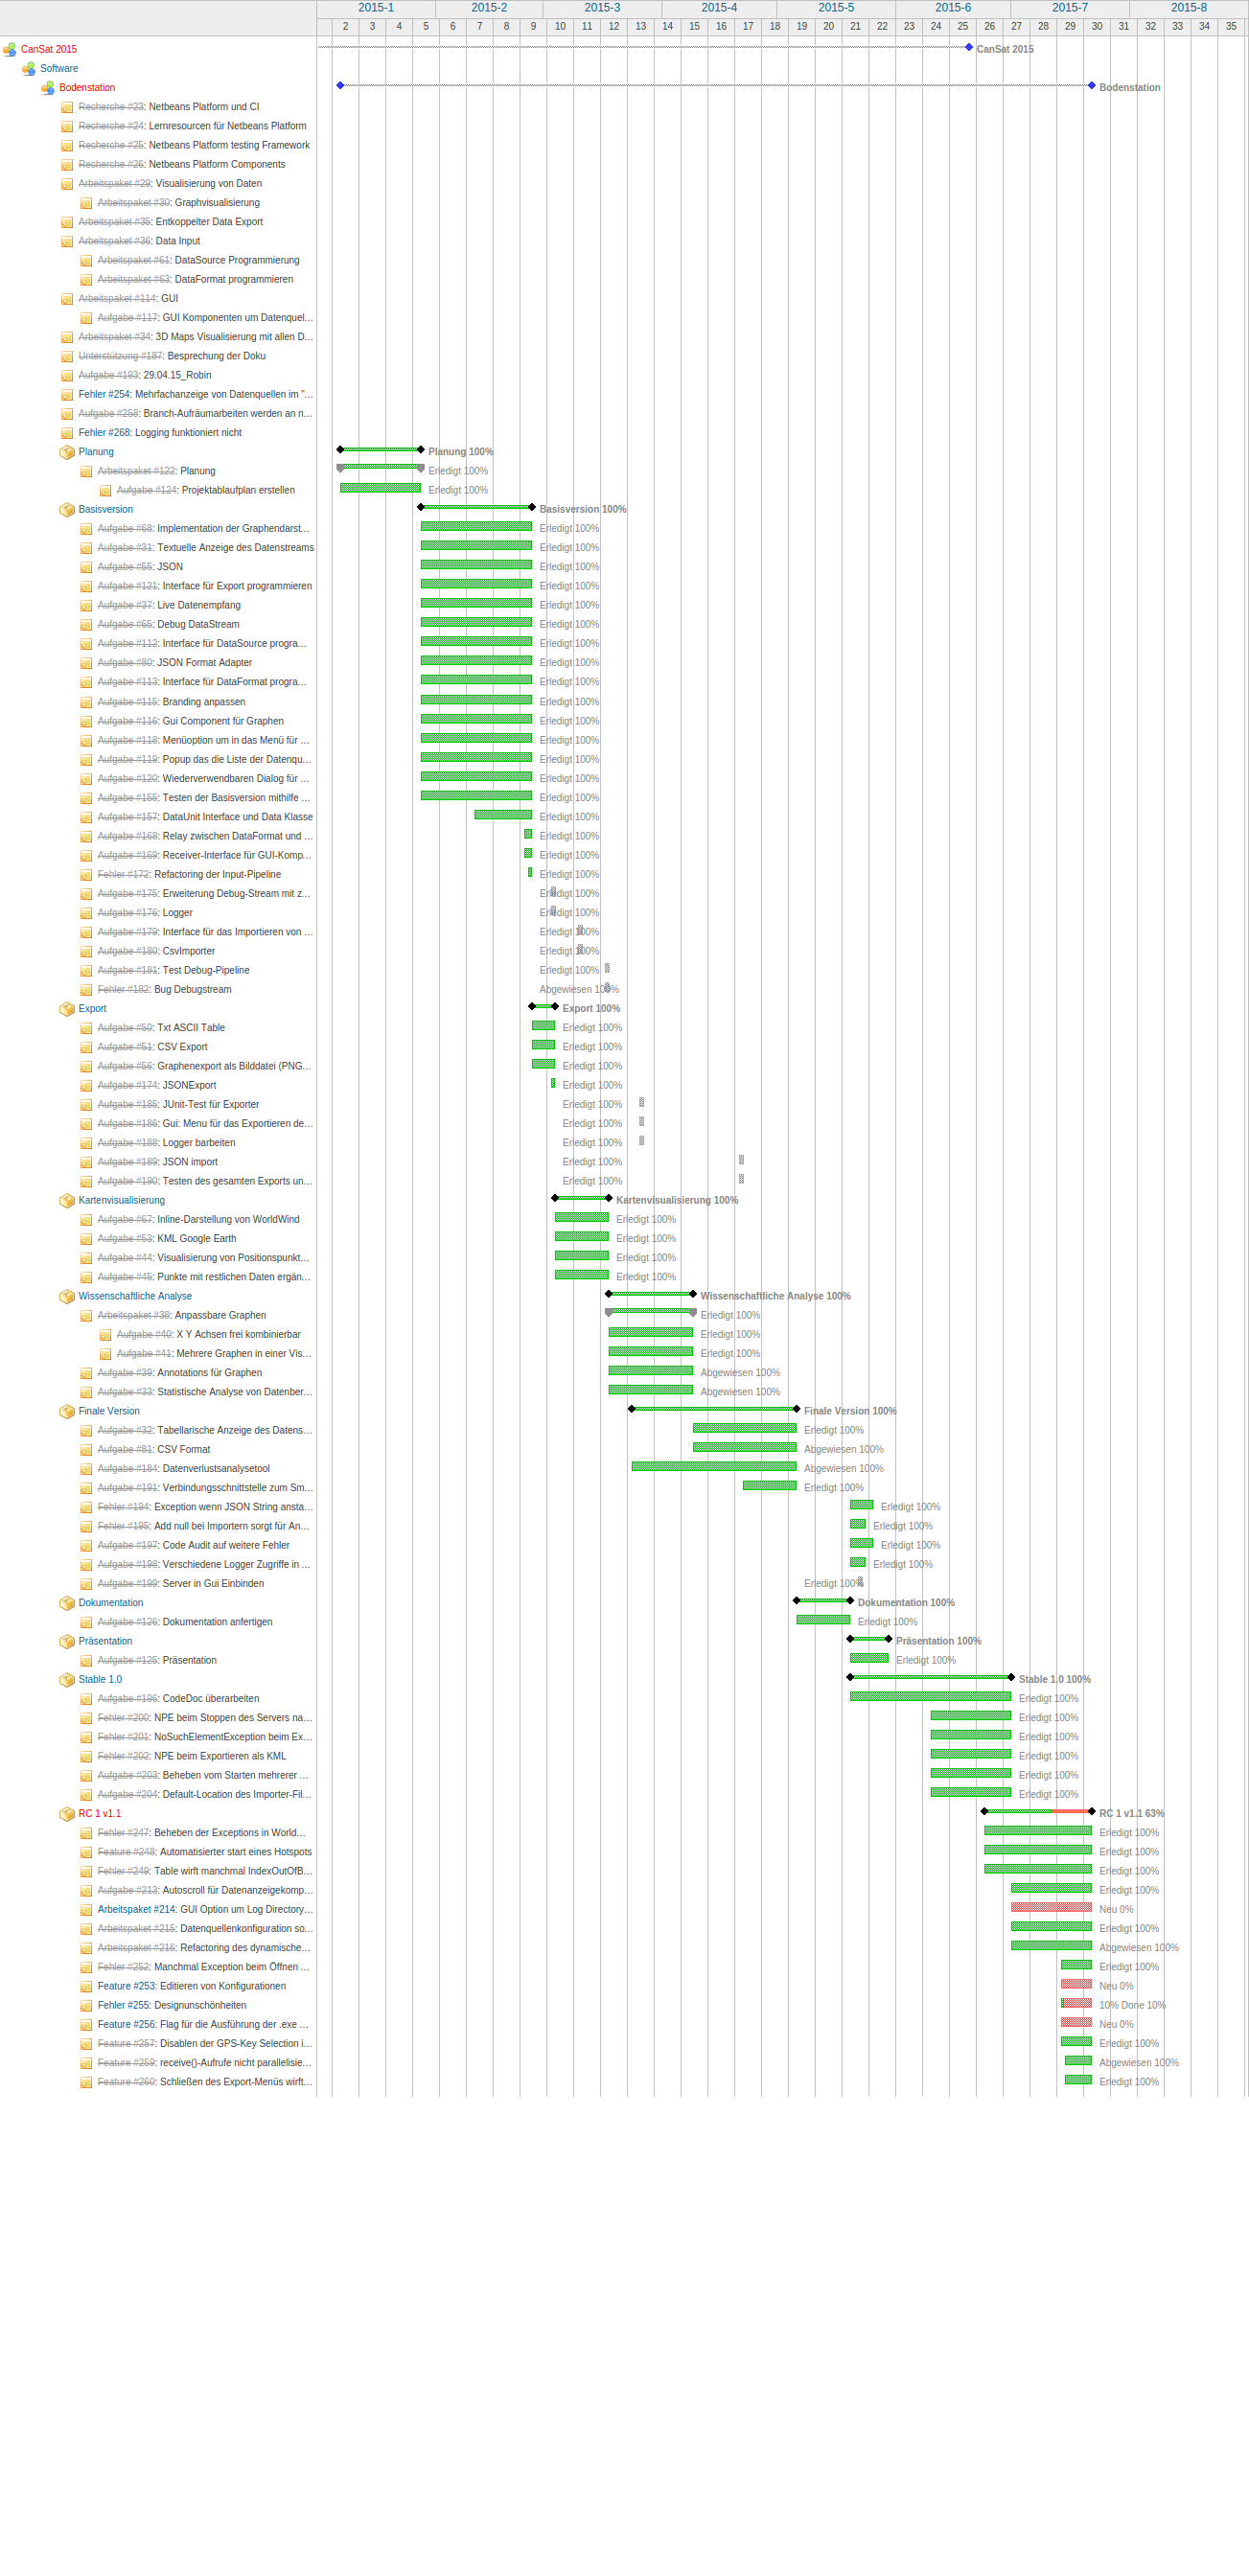
\includegraphics[width=0.7\textwidth]{8_Anhang/software-gantt.png}
	\caption{Das GANTT-Diagramm der Bodenstation}
	\label{gantt_software}
\end{figure}
\newpage
\subsubsection {Android-App-GANTT}
\begin{figure}[H]
	\centering
	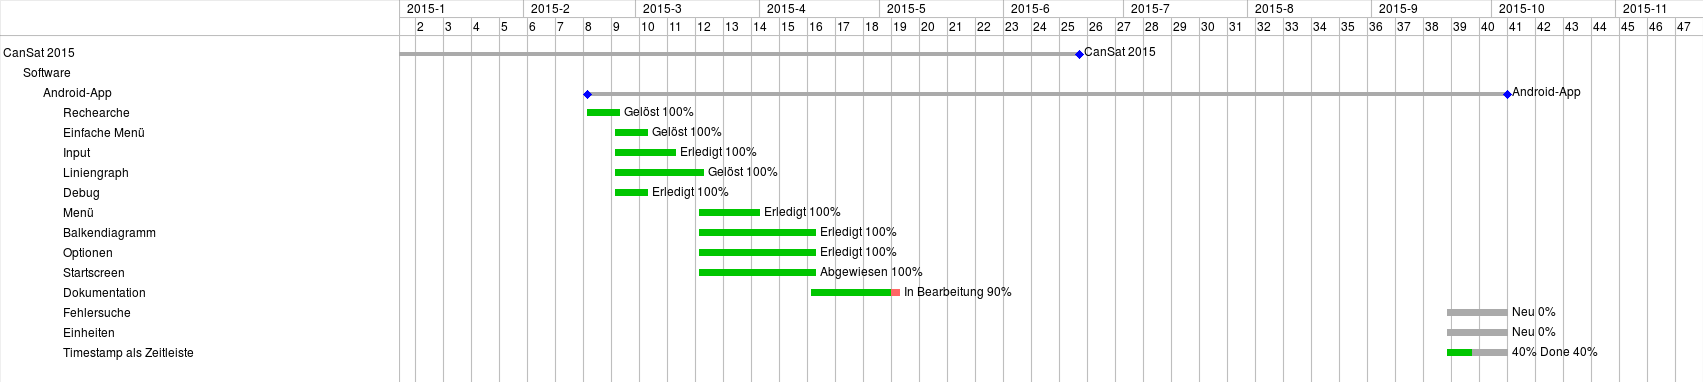
\includegraphics[width=0.8\textwidth]{8_Anhang/android-app-gantt.png}
	\caption{Das GANTT-Diagramm der Android-App}
	\label{gantt_android}
\end{figure}

\newpage
\subsection{Der CanSat}

\begin{figure}[H]
	\centering
	\includegraphics[trim = 11mm 335mm 20mm 210mm, clip, width=0.8\textwidth]{8_Anhang/dose.jpg}
	\caption{Die Hülle und ein Dosendeckel}
	\label{pic_dose}
\end{figure}

\begin{figure}[H]
	\centering
	\includegraphics[ width=0.8\textwidth]{8_Anhang/Wand_3D.PNG}
	\caption{Screenshot der Zwischenwand aus Sketchup}
	\label{pic_wand_3d}
\end{figure}

\newpage

\begin{figure}[h] 
      \centering 
      \includemovie[ 
        poster,controls,
       3Djscript=2_Beschreibung_des_CANSAT/Encompass.js
      ]{0.8\textwidth}{15cm}{2_Beschreibung_des_CANSAT/CanSat_2015.u3d} 
      \caption{Der Satellit (Diese Zeichnung ist möglicherweiße nicht sichtbar, da es eine 3D-Zeichnung ist. Bitte verwenden Sie den \href{https://get.adobe.com/reader/?loc=de}{Adobe Acrobat Reader})}\label{pic_3d} 
\end{figure} 

\newpage

\begin{figure}[H]
	\centering
	\includegraphics[trim = 60mm 100mm 55mm 100mm, clip, width=0.8\textwidth]{8_Anhang/Schaltplanv1.png}
	\caption{Der Schaltplan der Sensorikplatine}
	\label{pic_schaltplan}
\end{figure}

\newpage

\begin{figure}[H]
	\centering
	\includegraphics[trim = 200mm 300mm 200mm 280mm, clip,width=0.8\textwidth]{8_Anhang/Layoutv1.png}
	\caption{Das Layout der Sensorikplatine}
	\label{pic_layout}
\end{figure}

\newpage

\begin{figure}[H]
	\centering
	\includegraphics[ width=0.8\textwidth]{8_Anhang/fallschirmSkizze.PNG}
	\caption{Skizze des Fallschirms}
	\label{pic_fallschrimskizze}
\end{figure}

\newpage

\subsection{Bodenstationsnutzeranleitung}
\label{bodenstationsanleitung}
\subsubsection{Datenempfang}
Um Daten in Echtzeit zu empfangen, muss eine Verbindung zu einem Satelliten aufgebaut werden. Hierzu muss generell zu allererst ein Satellit erstellt werden. Hierfür wählt man unter dem Menüpunkt ``File'' den Unterpunkt ``Satellites'' aus. Dort ist es möglich, unter ``Add'', einen Satelliten hinzuzufügen. Um einen Satelliten zu laden, wählt man im selben Unterpunkt ``Manage'' aus. Dort wählt man den Satelliten aus, von welchem man Daten empfangen will. Anschließend sieht man einen Dialog mit Konfigurationsmöglichkeiten für den Datenempfang vom Satelliten (z. B. Serieller Port). Wenn man die Konfiguration abgeschlossen hat, beendet man den Dialog mit einem Klick auf ``Load configuration''. 
Möchte man den Datenempfangen beginnen, dann klickt man auf den ``Play''-Button in der Toolbar, welcher die Datenübertragung startet. Ab hier können verschiedene Visualisierungen geöffnet werden, um die empfangenen Daten darzustellen.
\subsubsection{Datenimport}
Um Daten aus einer Datei zu importieren, wird im Menüpunkt ``File'' der Untermenüpunkt ``Import'' ausgewählt. Anschließend wird eine Datei ausgewählt, welche importiert werden soll. Mit der Bestätigung werden die Daten dieser Datei eingelesen.
\subsubsection{Datenexport}
Für das Exportieren der Daten gilt, dass alle aktuell geladenen Daten exportiert werden. Darunter fallen entweder zwischengespeicherte Daten einer Liveübertragung, oder Daten, welche aus einer Datei importiert wurden.
Zum Exportieren der Daten wird im Menüpunkt ``File'' der Untermenüpunkt ``Export'' ausgewählt. Unter diesem Menüpunkt ist das Datenformat wählbar, in welches die gesammelten Daten gespeichert werden (Beim Graphenexport ist es wichtig, dass die Graphenvisualisierung während des Vorgangs geöffnet ist). Anschließend ist ein Pfad und ein Name wählbar, unter dem die Datei gespeichert wird. Mit der Bestätigung werden die Daten exportiert.
\subsubsection{Datenweiterleitung}
Per Klick auf das rote runde Icon in der Toolbar wird ein Hotspot-Server gestartet. Dieser sendet empfangene Daten in Echtzeit an alle Clients weiter, die mit dem Hotspot-Server verbunden sind.
\subsubsection{Oberflächenpersonalisierung}
Der Oberfläche können einzelne Komponenten hinzugefügt und entfernt werden. Diese Komponenten können unterschiedlich angeordnet werden. Um Visualisierungs-Komponenten hinzuzufügen wird unter dem Menü ``Window'' eine Visualisierung ausgewählt.
Um einen der bestehenden Komponenten zu entfernen wird das Kreuz angeklickt, welches sich am Tab des Komponenten befindet. Per ``drag and drop''  können diese Komponenten neu angeordnet werden, dazu muss der Tab des Komponenten ausgewählt werden. In verschiedenen Bereichen können Komponenten angeheftet oder verschoben werden. Außerdem können diese übereinander verlagert werden um sie in verschiedenen Tabs und in dem selben Bereich zu verwalten.

\subsubsection{Kartenvisualisierung}
Die Kartenvisualisierung startet über den Untermenüpunkt ``Map Visualization'' im Menüpunkt ``Window''. Geladene Werte werden dort angezeigt. Einzelne Messpunkte sind mit einem Punkt gekennzeichnet und mit einer Linie verbunden, was den Flugweg des Satelliten anzeigt.

\subsubsection{Graphenvisualisierung}
Um einen Graphen zu erzeugen, wählt man unter dem Menüpunkt ``Window'' - ``Graph Visualization'' aus. Anschließend wird in der Oberfläche ein Graph erzeugt. Die Achsen des Graphs sind mit Sensorwerten belegbar. Um die Belegung der Achsen zu verändern, wählt man an den Achsen den jeweiligen Sensor aus und drückt den Button ``Refresh axes''.

\subsubsection{Textdarstellung}
Zusätzlich können die empfangenen Daten auch direkt dargestellt werden, indem man den Menüpunkt ``Window'' - ``Text Stream'' auswählt.

\subsubsection {Tabellendarstellung}
Die empfangenen Daten können ebenfalls in einer Tabelle dargestellt werden, welche über den Menüpunkt ``Table Visualization'' geöffnet werden kann.

\subsubsection{Fenster zurücksetzen}
Die Anordnung der Komponenten der Oberfläche kann im Menüpunkt ``Window'' unter ``Reset Windows'' zurückgesetzt werden.

\subsubsection{Beenden des Programms}
Um das Programm zu beenden, gibt es zwei Möglichkeiten. Zum einen wird das Programm beendet, wenn das Kreuz am oberen rechten Rand der Oberfläche angeklickt wird. Zum anderen kann das Programm über den Menüpunkt ``File'' geschlossen werden, in dem man dort ``Exit'' auswählt.

